\begin{frame}%[t]
  \frametitle{Finite Element Approximations}
  \begin{itemize}
    \item{Many different finite element pairs have been tried \ldots}
    \item{
  \only<1>
      {
	$P_1^{NC}-P_1$
	\begin{center}
	  \includegraphics[width=.4\textwidth,angle=-90]{figures/P1NCP1}
	\end{center}
      }
      %
%%   \only<2>
%%       {
%% 	$P_2-P_1$
%% 	\begin{center}
%% 	  \includegraphics[width=.4\textwidth,angle=-90]{figures/P2P1}
%% 	\end{center}
%%       }
      %
  \only<2>
      {
	$P_1-P_1$
	\begin{center}
	  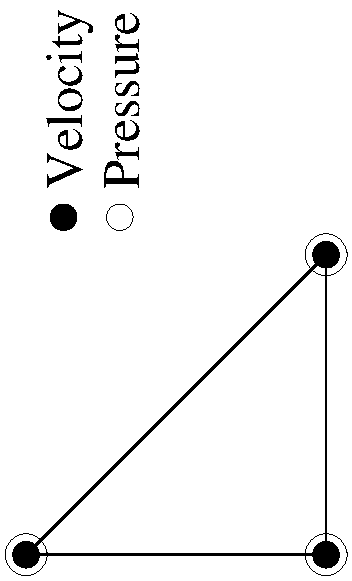
\includegraphics[width=.4\textwidth,angle=-90]{figures/P1P1}
	\end{center}
      }
      %
  \only<3>
      {
	$P_0-P_1$
	\begin{center}
	  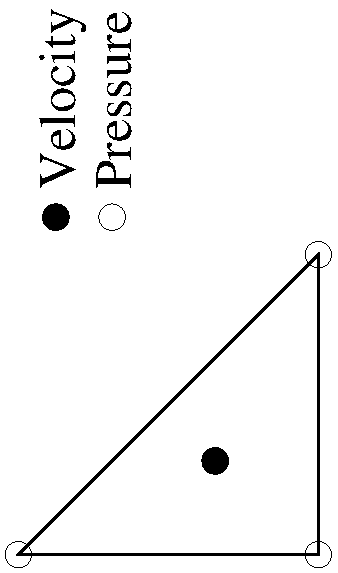
\includegraphics[width=.4\textwidth,angle=-90]{figures/P0P1}
	\end{center}
      }
%%   \only<5>
%%       {
%% 	$RT0$
%% 	\begin{center}
%% 	  \includegraphics[width=.4\textwidth,angle=-90]{figures/RT0}
%% 	\end{center}
%%       }
    }
  \end{itemize}
\end{frame}


\begin{frame}%[t]
  \frametitle{FE-pair advantages/disadvantages}
  \begin{itemize}%[<+->]
%  \item{Each FE-pair has various advantages/disadvantages, for example}
    \only<1>
    {
    \item{
      $P_1^{NC}-P_1$
      \begin{itemize}
	\item {$+$ ``A promising choice for the discretization of a variety
	  of coastal and environmental problems'' (Le~Roux, 2005)}
	\item {$-$ Difficult to use in $h$-adaptive codes with hanging nodes and
	  nested spaces}
      \end{itemize}
      }
      }
    \only<2>
    {
    \item{
      $P_1-P_1$
      \begin{itemize}
	\item {$+$ Simple implementation, elements work fine in $h$-adaptive codes}
	\item {$-$ ``Spurious modes of wavelength $3h$ are present'' for gravity
	  wave propagation problems with non-constant bathymetry (Le~Roux, 2007)}
	\item{$-$ ``the $P_1-P_1$ pair is usually not used to solve the SW system, unless
	  \ldots a stabilization procedure is employed'' (\emph{ibid})}
      \end{itemize}
      }
      }
    \only<3>
    {
    \item{
      $P_0-P_1$
      \begin{itemize}
	\item {$+$ No spurious elevation modes as for $P_1-P_1$}
	\item {$-$ Actually \emph{more} expensive than $P_1-P_1$ on an equivalent mesh}
	\item {$-$ Only weak enforcement of velocity BCs is possible since there are no
	  velocity dofs on the element edges}
      \end{itemize}
      }
      }
  \end{itemize}
\end{frame}
